\documentclass[10pt]{beamer}
\usepackage{xeCJK}
\usepackage[utf8]{inputenc}
% \usepackage{xeCJK} % Disabled to avoid Fandol font error
\usepackage{graphicx}
\usepackage {mathtools}
\usepackage[inkscapeformat=png]{svg}
\usepackage{utopia} %font utopia imported
\usetheme{CambridgeUS}
% \usepackage{fontspec}
\usepackage{tikz}
\usetikzlibrary{positioning,calc}
\usetikzlibrary{positioning,arrows.meta,calc}
% \usepackage{fourier}  % sans serif font
\renewcommand{\familydefault}{\sfdefault}
\usecolortheme{dolphin}
\usepackage[backend=biber,style=numeric]{biblatex}
\addbibresource{bibliography.bib} % Ensure bibliography.bib exists and contains at least one entry with key 'example_reference'

% set colors to University of Kassel colours
\definecolor{myNewColorA}{RGB}{172,4,76}
\definecolor{myNewColorB}{RGB}{197,83,132}
\definecolor{myNewColorC}{RGB}{209,145,173}
\setbeamercolor*{palette primary}{bg=myNewColorC}
\setbeamercolor*{palette secondary}{bg=myNewColorB, fg = white}
\setbeamercolor*{palette tertiary}{bg=myNewColorA, fg = white}
\setbeamercolor*{titlelike}{fg=myNewColorA}
\setbeamercolor*{title}{bg=myNewColorA, fg = white}
\setbeamercolor*{item}{fg=myNewColorA}
\setbeamercolor*{caption name}{fg=myNewColorA}
\usefonttheme{professionalfonts}
\usepackage{hyperref}
\usepackage[printonlyused]{acronym}
% \usepackage[nolist]{acronym}    


%------------------------------------------------------------
\titlegraphic{
\includegraphics[height=1.5cm]{images/Logo_Uni_Kassel.png}}
\newcommand{\university}{University of Kassel}
\setbeamerfont{title}{size=\large}
\setbeamerfont{subtitle}{size=\small}
\setbeamerfont{author}{size=\small}
\setbeamerfont{date}{size=\small}
\setbeamerfont{institute}{size=\small}
% \setbeamerfont{instituteB}{size=\small}
\title[\university{}]{Conceptual Topic Aggregation}
\subtitle{A Case Study on the ETYNTKE Dataset}
\author[Klara M. Gutekunst]{Klara M. Gutekunst \and Dominik Dürrschnabel \and Gerd Stumme \and Johannes Hirth}

\institute[klara.gutekunst@uni-kassel.de]{\university{}}
% \instituteB[KDE]{\inst{2}Knowledge and Data Engineering Group
% Department of Electrical Engineering and Computer Science
% Interdisciplinary Research Center for Information System Design
% University of Kassel}
\date[\today]
{\today}

%------------------------------------------------------------
%This block of commands puts the table of contents at the 
%beginning of each section and highlights the current section:
%\AtBeginSection[]
%{
%  \begin{frame}
%    \frametitle{Contents}
%    \tableofcontents[currentsection]
%  \end{frame}
%}
\AtBeginSection[]{
  \begin{frame}
  \vfill
  \centering
  \begin{beamercolorbox}[sep=8pt,center,shadow=true,rounded=true]{title}
    \usebeamerfont{title}\insertsectionhead\par%
  \end{beamercolorbox}
  \vfill
  \end{frame}
}
%------------------------------------------------------------

\begin{document}
% \setmainfont{Crimson Pro}

%The next statement creates the title page.
\frame{\titlepage}
\begin{frame}
\frametitle{Contents}
\tableofcontents
\end{frame}
%------------------------------------------------------------
\section{Motivation}
\begin{frame}{Motivation}
    \only<1>{
        \begin{figure}
            \includesvg[width=\linewidth]{images/steps/overview.svg}
        \end{figure}
    } 
    \only<2>{
        \begin{figure}
            \includesvg[width=\linewidth]{images/steps/overview_step1.svg}
        \end{figure}
    } 
    \only<3>{
        \begin{figure}
            \includesvg[width=\linewidth]{images/motivation/motivation1.svg}
        \end{figure}
    }
    \only<4>{
        \begin{figure}
            \includesvg[width=\linewidth]{images/motivation/motivation2.svg}
        \end{figure}
    }
    \only<5>{
        \begin{figure}
            \includesvg[width=\linewidth]{images/motivation/motivation3.svg}
        \end{figure}
    }
\end{frame}

\begin{frame}{Motivation} 
    \begin{columns}
        \begin{column}{0.8\textwidth}
            \begin{alertblock}{Problem} 
            Employees at the tax office often lack prior knowledge about the contents of the data before starting exploration.
            \end{alertblock}

            \visible<2->{What is our objective?\\}
            \visible<3->{$\rightarrow$ \textbf{Gain an initial understanding of the data.}}
        \end{column}
        \begin{column}{0.18\textwidth}
            \begin{figure}
                \centering
                
\includegraphics[width=0.7\textwidth]{images/motivation/tax.png}
            \end{figure}
        \end{column}
    \end{columns}
\end{frame}


\begin{frame}{Motivation} 
    \begin{exampleblock}{Objective} 
    Gain an initial understanding of the data.
    \end{exampleblock}

    \visible<2->{\textbf{Challenges:}}
    \begin{itemize}
        \item[\ding{55}]<3-> Lack of labeled data for supervised training
        \item[\ding{55}]<4-> Diverse data formats and structures
    \end{itemize}

    \visible<5->{How did we tackle these problems?}
    \begin{itemize}
        \item[\ding{51}]<6-> Fully unsupervised analysis pipeline
        \item[\ding{51}]<7-> Handles multiple languages and file types
    \end{itemize}
\end{frame}
\section{Dataset}

\begin{frame}{Everything You Need To Know Ever\footnote{\url{https://archive.org/details/ETYNTKE} (29.01.2025)}}
    \begin{columns}[T] % align top
        \begin{column}{0.6\textwidth}
             \begin{itemize}
                \item Approx. 101 GB 
                \item Images, text documents, and other file types
                \item Malformed files
                \item Uploaded in 2015
                \item Topics include politics, weaponry, and Computer Science
                \item Hierarchical organization into directories
            \end{itemize}
        \end{column}

        \begin{column}{0.3\textwidth}
            \begin{figure}
                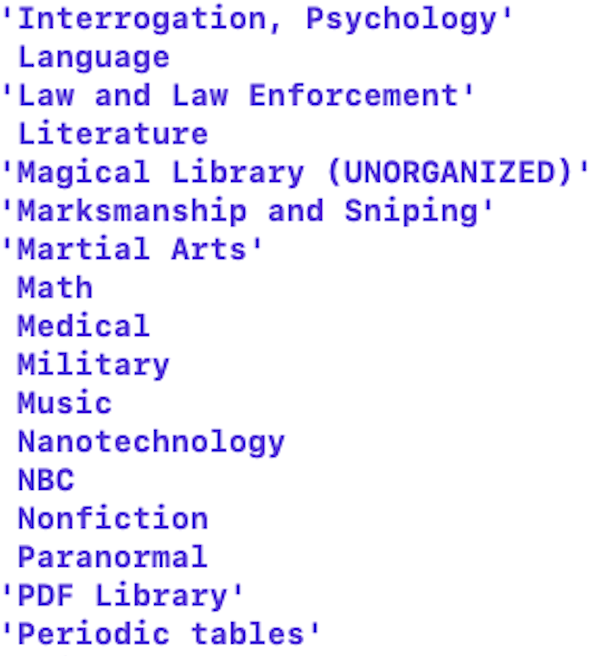
\includegraphics[width=\linewidth]{images/screenshot_data.png}
                \caption{Subset of top-level directories in the ETYNTKE dataset.} % replaces \caption
            \end{figure}
   
        \end{column}
    \end{columns}
\end{frame}


\section{Mathematical Foundations}
\begin{frame}{\acf{fca}~\parencite{fca-book}} 
    
\begin{description}
    \item[Formal context] $\mathbb{K} \coloneq (G, M, I)$
    \begin{itemize}
        \item $G$ object set
        \item $M$ attribute set
        \item $I \subseteq G \times M$ incidence relation
    \end{itemize}
\item [Derivation operations] \text{ }
\begin{itemize}
    \item For $A \subseteq G $: $A' \coloneq \{m \in M \mid (g, m) \in I \text{ } \forall g \in A \}$
    %object derivation $(\cdot)' : \mathcal{P}(G) \to \mathcal{P}(M)$
    \item For $B \subseteq M $: $B' \coloneq \{g \in G \mid (g, m) \in I \text{ } \forall m \in B\}$
\end{itemize}
\item [Formal concepts] $\mathfrak{B}(\mathbb{K}) \coloneq \{(A,B) | A' = B \land B' = A \}$ 
\begin{itemize}
    \item $A \subseteq G$ and $B \subseteq M$
\end{itemize} 
\item [Concept lattice] $\underline{\mathfrak{B}}(\mathbb{K}) \coloneq (\mathfrak{B}(\mathbb{K}), \leq)$ with $(A_1, B_1) \leq (A_2, B_2) \iff A_1 \subseteq A_2$.
\begin{itemize}
    \item $A_i \subseteq G$ and $B_i \subseteq M$
\end{itemize} 
\end{description}
\end{frame}

\newcommand{\FormalConceptGraph}{%
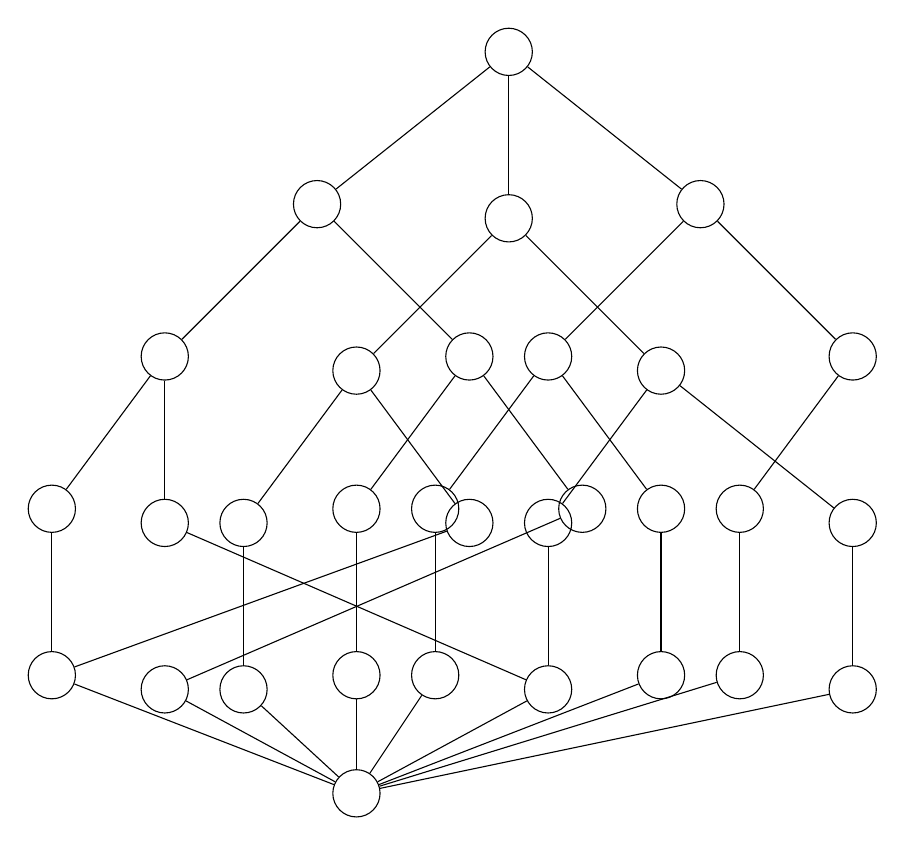
\begin{tikzpicture}[
    concept/.style={
        circle, draw, minimum size=6mm, inner sep=1mm
    },
    level distance=15mm
]
    
    % Layer 0 (top)
    \node[concept] (n0) {};

    % Layer 1
    \node[concept, below left=15mm and 20mm of n0] (n1) {};
    \node[concept, below=15mm of n0] (n2) {};
    \node[concept, below right=15mm and 20mm of n0] (n3) {};

    % Layer 2
    \node[concept, below left=15mm and 15mm of n1] (n4) {};
    \node[concept, below right=15mm and 15mm of n1] (n5) {};
    \node[concept, below left=15mm and 15mm of n2] (n6) {};
    \node[concept, below right=15mm and 15mm of n2] (n7) {};
    \node[concept, below left=15mm and 15mm of n3] (n8) {};
    \node[concept, below right=15mm and 15mm of n3] (n9) {};

    % Layer 3
    \node[concept, below left=15mm and 10mm of n4] (n10) {};
    \node[concept, below=15mm and 10mm of n4] (n11) {};
    \node[concept, below left=15mm and 10mm of n5] (n12) {};
    \node[concept, below right=15mm and 10mm of n5] (n13) {};
    \node[concept, below left=15mm and 10mm of n6] (n14) {};
    \node[concept, below right=15mm and 10mm of n6] (n15) {};
    \node[concept, below left=15mm and 10mm of n7] (n16) {};
    \node[concept, below=15mm and 10mm of n9] (n17) {};
    \node[concept, below left=15mm and 10mm of n8] (n18) {};
    \node[concept, below right=15mm and 10mm of n8] (n19) {};
    \node[concept, below left=15mm and 10mm of n9] (n20) {};

    % Layer 4 (bottom)
    \node[concept, below=15mm of n10] (n22) {};
    \node[concept, below=15mm of n12] (n23) {};
    \node[concept, below=15mm of n14] (n24) {};
    \node[concept, below=15mm of n16] (n25) {};
    \node[concept, below=15mm of n18] (n26) {};
    \node[concept, below=15mm of n20] (n27) {};
    \node[concept, below=15mm of n11] (n28) {};
    \node[concept, below=15mm of n17] (n29) {};
    \node[concept, below=15mm of n19] (n30) {};

    % Single bottom node
    \node[concept] (n31) at ($ (n22)!0.5!(n30) + (0,-15mm) $) {};
    % \node[concept] (n31) at ($(n22)!0.5!(n30) - (0,15mm)$) {};
    % \node[concept, below=15mm of $(n22)!0.5!(n30)$] (n31) {};

    % Draw downward edges only
    \foreach \from/\to in {
        n0/n1, n0/n2, n0/n3,
        n1/n4, n1/n5, n2/n6, n2/n7, n3/n8, n3/n9,
        n4/n10, n4/n11, n5/n12, n5/n13, n6/n14, n6/n15, n7/n16, n7/n17, n8/n18, n8/n19, n9/n20, 
        n10/n22, n11/n25, n12/n23, n13/n28, n14/n24, n15/n22, n16/n25, n17/n29, n18/n26, n19/n30, n20/n27}
    {
        \draw (\from) -- (\to);
    }

    % Connect all bottom layer nodes to the single bottom node
    \foreach \n in {n22,n23,n24,n25,n26,n27,n28,n29,n30}
    {
        \draw (\n) -- (n31);
    }

\end{tikzpicture}%
}


\newcommand{\FormalConceptGraphColoured}{%
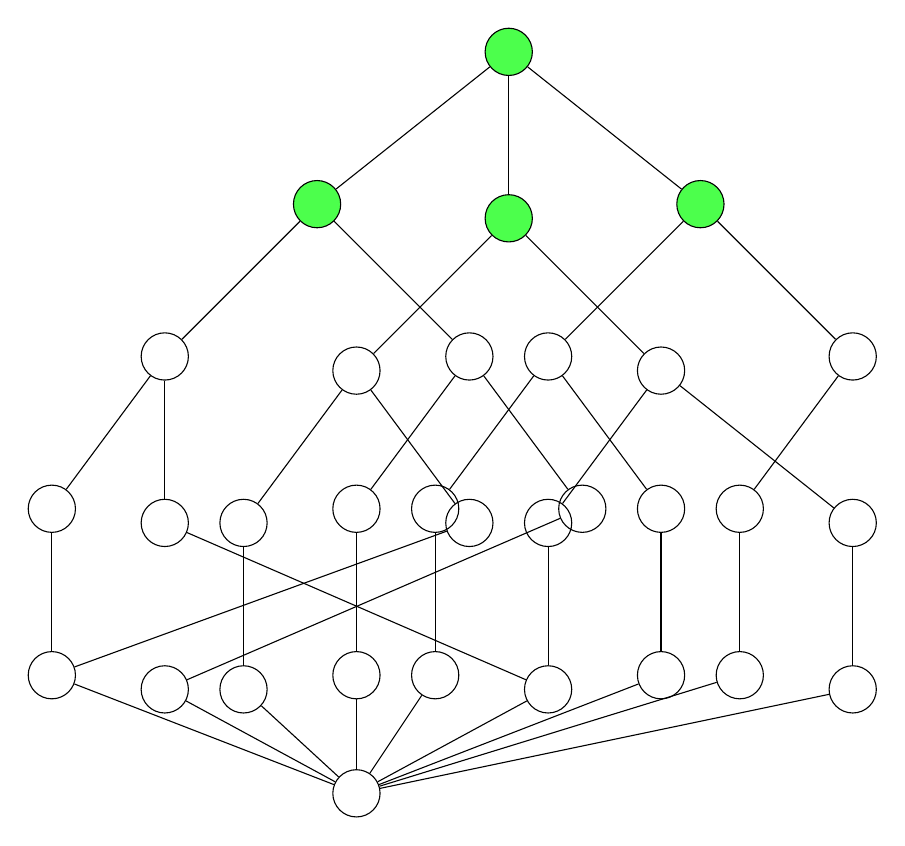
\begin{tikzpicture}[
    concept/.style={
        circle, draw, minimum size=6mm, inner sep=1mm
    },
    level distance=15mm
]

% Layer 0
\node[concept, fill=green!70] (n0) {};

% Layer 1
\node[concept, below left=15mm and 20mm of n0, fill=green!70] (n1) {};
\node[concept, below=15mm of n0, fill=green!70] (n2) {};
\node[concept, below right=15mm and 20mm of n0, fill=green!70] (n3) {};

   % Layer 2
    \node[concept, below left=15mm and 15mm of n1] (n4) {};
    \node[concept, below right=15mm and 15mm of n1] (n5) {};
    \node[concept, below left=15mm and 15mm of n2] (n6) {};
    \node[concept, below right=15mm and 15mm of n2] (n7) {};
    \node[concept, below left=15mm and 15mm of n3] (n8) {};
    \node[concept, below right=15mm and 15mm of n3] (n9) {};

    % Layer 3
    \node[concept, below left=15mm and 10mm of n4] (n10) {};
    \node[concept, below=15mm and 10mm of n4] (n11) {};
    \node[concept, below left=15mm and 10mm of n5] (n12) {};
    \node[concept, below right=15mm and 10mm of n5] (n13) {};
    \node[concept, below left=15mm and 10mm of n6] (n14) {};
    \node[concept, below right=15mm and 10mm of n6] (n15) {};
    \node[concept, below left=15mm and 10mm of n7] (n16) {};
    \node[concept, below=15mm and 10mm of n9] (n17) {};
    \node[concept, below left=15mm and 10mm of n8] (n18) {};
    \node[concept, below right=15mm and 10mm of n8] (n19) {};
    \node[concept, below left=15mm and 10mm of n9] (n20) {};

    % Layer 4 (bottom)
    \node[concept, below=15mm of n10] (n22) {};
    \node[concept, below=15mm of n12] (n23) {};
    \node[concept, below=15mm of n14] (n24) {};
    \node[concept, below=15mm of n16] (n25) {};
    \node[concept, below=15mm of n18] (n26) {};
    \node[concept, below=15mm of n20] (n27) {};
    \node[concept, below=15mm of n11] (n28) {};
    \node[concept, below=15mm of n17] (n29) {};
    \node[concept, below=15mm of n19] (n30) {};

    % Single bottom node
    \node[concept] (n31) at ($ (n22)!0.5!(n30) + (0,-15mm) $) {};
    % \node[concept] (n31) at ($(n22)!0.5!(n30) - (0,15mm)$) {};
    % \node[concept, below=15mm of $(n22)!0.5!(n30)$] (n31) {};

    % Draw downward edges only
    \foreach \from/\to in {
        n0/n1, n0/n2, n0/n3,
        n1/n4, n1/n5, n2/n6, n2/n7, n3/n8, n3/n9,
        n4/n10, n4/n11, n5/n12, n5/n13, n6/n14, n6/n15, n7/n16, n7/n17, n8/n18, n8/n19, n9/n20, 
        n10/n22, n11/n25, n12/n23, n13/n28, n14/n24, n15/n22, n16/n25, n17/n29, n18/n26, n19/n30, n20/n27}
    {
        \draw (\from) -- (\to);
    }

    % Connect all bottom layer nodes to the single bottom node
    \foreach \n in {n22,n23,n24,n25,n26,n27,n28,n29,n30}
    {
        \draw (\n) -- (n31);
    }


\end{tikzpicture}%
}





%%%%%%%%%%%%%%%%%%%%%%%%%%%%%%%%%%%%%%%%%%%%%%%
\begin{frame}{TITANIC~\cite{titanic_2002}}
\begin{columns}
\begin{column}{0.7\textwidth}
\begin{alertblock}{Problem} % with large datasets
The size of a concept lattice can grow exponentially with respect to the size of the context.
\end{alertblock}

\visible<2->{
    \begin{exampleblock}{Solution}
    Consider only top-level concepts.
    \end{exampleblock}
}
\end{column}

\begin{column}{0.25\textwidth}

\only<1>{
\begin{figure}[htbp]
    \centering
    \resizebox{\textwidth}{!}{\FormalConceptGraph}
    \caption{Concept lattice.}
    \label{fig:titanic_formal_concept_graph}
\end{figure}
}

\only<2->{
\begin{figure}[htbp]
    \centering
    \resizebox{\textwidth}{!}{\FormalConceptGraphColoured}
    \caption{Concept lattice.}
    \label{fig:titanic_formal_concept_graph_iceberg}
\end{figure}
}



\end{column}
\end{columns}
\end{frame}


\begin{frame}{TITANIC~\cite{titanic_2002}}
\begin{definition}
Support $supp(B) = \frac{\left| B' \right|}{\left| G \right|}$
\end{definition}


\begin{description}
    \item<2->[minimum support] $minsupp \in [0,1]$: Threshold below which attribute sets are not considered frequent
    \item <3-> [frequent attribute set] $B \subseteq M$: $supp(B) \ge minsupp$  % in $\mathbb{K}$ if
    \item <4-> [frequent concept] $(A, B)$: $B$ is frequent attribute set
\end{description}

    



\end{frame}

\begin{frame}{TITANIC~\cite{titanic_2002}}
\begin{columns}
    \begin{column}{0.7\textwidth}
        \begin{definition}
        The iceberg concept lattice of a context $\mathbb{K}$ comprises all frequent concepts.
        \end{definition}

        \visible<2->{
        \begin{description}
            \item[TITANIC] algorithm computes iceberg concept lattices.
        \end{description}
        % An iceberg concept lattice includes only the top-level concepts, specifically those corresponding to frequent attribute sets.
        }
    \end{column}
    \begin{column}{0.25\textwidth}
    \begin{figure}[htbp]
        \centering
        \resizebox{\textwidth}{!}{\FormalConceptGraphColoured}
        \caption{Iceberg concept lattice coloured.}
        \label{fig:titanic_formal_concept_graph_coloured}
    \end{figure}
    \end{column}
\end{columns}
\end{frame}

\section{Topic modelling}

\begin{frame}{Topic modelling}
How do text topic modelling techniques uncover latent topics in leaked documents?

How well do different topic modelling techniques perform on leaked document datasets, considering their suitability and effectiveness?
\end{frame}

\section{\acs{fca} Topic Aggregation}
    \begin{frame}{\acs{fca} Topic Aggregation}
    Can \acs{fca} tools produce a hierarchical description of the semantic similarities of directories in the dataset?
    \end{frame}



\section{Conclusion}
    \begin{frame}{Conclusion}
    \end{frame}



\section*{Acknowledgement}  
\begin{frame}
\textcolor{myNewColorA}{\Huge{\centerline{Thank you!}}}
\end{frame}


\begin{frame}[allowframebreaks]
\frametitle{References}
Here is an example citation~\cite{example_reference}.
\printbibliography
\end{frame}

\section*{List of abbreviations}

\begin{acronym}[XXXXXXXXX]
    \acro{fca}[FCA]{Formal Concept Analysis}
    \acro{dataset}[ETYNTKE]{Everything You Need To Know Ever}
    \acro{nlp}[NLP]{Natural Language Processing}
    \acro{git}[GIT]{Generative Image-to-text Transformer}
    \acro{pdf}[PDF]{Portable Document Format}
    \acro{ner}[NER]{Named Entity Recognition}
    \acro{ne}[NE]{Named Entity}
    \acro{sbert}[SBERT]{Sentence-BERT}
    \acro{use}[USE]{Universal Sentence Encoder}
    \acro{es}[ES]{Elasticsearch}
    \acro{umap}[UMAP]{Uniform Manifold Approximation and Projection for Dimension Reduction}
    \acro{tsne}[t-SNE]{t-Distributed Stochastic Neighbor Embedding}
    \acro{pca}[PCA]{Principal Component Analysis}
    \acro{hdbscan}[HDBSCAN]{Hierarchical Density-Based Spatial Clustering of Applications with Noise}
    \acro{bow}[BoW]{Bag of Words}
    \acro{tfidf}[TF-IDF]{Term Frequency-Inverse Document Frequency}
    \acro{approachname}[FAT-CAT]{FCA-based Aggregation for Topics using Conceptual Analysis and Taxonomies}
    \acro{cne}[CNE]{Clustering Named Entities}
    \acro{edr}[EDR]{Embedding - Dimension Reduction}
    \acro{hlda}[hLDA]{Hierarchical Latent Dirichlet Allocation}

    % \acro{}[]{}
\end{acronym}
\end{document}



